\chapter{Implementation Details}

This chapter describes the implementation of the proposed visual geolocation system. The system is implemented as a sequence of software modules. Each module performs one specific task and passes its output to the next stage.

The complete implementation contains five main components. These are the reference skyline database generation, synthetic dataset generation, sky segmentation, skyline extraction, and skyline matching modules. The final evaluation module measures the localization performance using generated query images and known ground truth locations.

\section{Reference Skyline Database Implementation}

The reference skyline database provides the collection of possible terrain skyline profiles used during localization. Each database entry represents a possible camera viewpoint inside the study area.

The database generation module takes the \gls{dem} file as input and samples viewpoints on a grid. Here, two distances must be separated clearly. The \gls{dem} raster has an approximate spatial resolution of 30~m, but the evaluation database used in this report is sampled at a 500~m viewpoint interval. The 30~m setting was used in initial local tests and sensitivity checks. The reported Chapter 6 results use the 500~m grid.

The 500~m viewpoint spacing was selected as a practical balance. It reduces computational cost, RAM usage, and database size while keeping matching speed high. In the Himalayas, skyline shape usually changes gradually over this distance, so the grid still preserves useful spatial detail.

For every viewpoint, the surrounding terrain is analysed up to a maximum distance of $30$~km. The visible terrain boundary is converted into a one-dimensional skyline profile.

The 30~km horizon radius was selected for this region because Himalayan valleys are strongly affected by terrain shielding. Beyond this range, Earth's curvature and atmospheric haze reduce visibility, and distant ridges add little stable detail. Viewshed analysis also showed that most useful skyline structure is already captured within 30~km.

The skyline is stored as elevation angles sampled at $1^\circ$ azimuth intervals. Therefore, each viewpoint contains a profile with 360 elevation values representing the complete horizontal view around the camera.

For each viewpoint, the terrain horizon is generated by finding the maximum elevation angle along each viewing direction. The elevation-angle computation follows \cref{eq:elevation_angle}. In this chapter, we use the shorthand $h = h_t - h_o$, so the same relation is written as $\theta = \tan^{-1}(h/d)$.

Not all generated viewpoints provide useful localization information. Flat regions and open areas can produce similar skyline shapes at many locations. To reduce these ambiguous cases, a profile-quality screening step is applied before profiles are stored.

This screening step removes profiles with very weak skyline information and keeps profiles with clearer terrain structure for matching.

The generated database is stored using the Parquet file format. Each record contains the viewpoint position and its corresponding skyline profile. The database format allows the matching module to access required rows without loading the complete dataset into memory.

\section{Synthetic Dataset Generation}

A synthetic dataset is generated to train and evaluate the skyline segmentation module. The dataset generation process creates mountain images together with their corresponding sky masks and camera information.

The terrain model is generated from the \gls{dem}. Satellite texture data is projected onto the terrain surface to provide realistic ground appearance. The rendering process produces images from different camera viewpoints selected from the terrain.

To increase image variation, different environmental conditions are applied during generation. The implemented presets include sunny, cloudy, sunset, storm, rainy, and night conditions. Each weather preset is generated by varying the lighting and sky colors, while procedural effects such as a randomly placed glowing sun, randomly placed star points, and random rain streaks are added where appropriate. Additional image effects such as sensor noise, vignette, lens flare, and chromatic effects are applied to simulate variations that may appear in real images.

The camera locations are randomly shifted from the original viewpoint grid positions. The displacement ranges from approximately $\pm1$~m to $\pm15$~m. This prevents the matching system from relying on exact database grid positions and allows evaluation of nearby locations.

For every rendered image, a corresponding binary sky mask is generated. The mask separates the sky region from the terrain region. Since the rendering environment is fully known, the generated masks provide accurate labels for model training.

The generated samples are stored in separate image and mask folders. The ground truth camera coordinates are stored separately and are used during evaluation.

Only 300 synthetic images were needed in this phase because the encoder was pretrained and did not start from scratch. Data augmentation increased visual diversity during training, and the synthetic set mainly supported domain adaptation to local Himalayan terrain appearance.

\section{Sky Segmentation Implementation}

The sky segmentation module extracts the sky region from a query image. The output of this module is a binary mask containing the sky and terrain boundary.

The segmentation model is implemented using a U-Net architecture with a MobileNetV3 encoder. The model receives an RGB image as input and produces a probability map representing the likelihood of each pixel belonging to the sky region.

U-Net was selected instead of DeepLabV3+ because this is a binary segmentation task and skyline boundary accuracy is critical. Its skip connections preserve edge detail from early layers, which helps keep ridge boundaries sharp. It also has lower computational cost for this use case.

MobileNetV3 was selected for smartphone deployment. It has low memory use and fast inference while maintaining good accuracy. This makes it suitable for offline field use on limited hardware.

Before inference, each image is resized to $256 \times 256$ pixels. The pixel values are normalized using the standard image normalization parameters used during model training.

The model output is converted into a binary mask using a threshold value of 0.5. The resulting mask is resized back to the original image resolution.

The initial segmentation result may contain small errors near the mountain boundary. These errors can occur because snow, clouds, and bright terrain regions may have similar appearance to the sky. To improve the boundary accuracy, an edge refinement process is applied.

First, connected component analysis is used to keep only sky regions connected to the top boundary of the image. This removes isolated incorrect regions.

Next, Canny edge detection is applied to the input image. The detected edges are used to adjust the predicted boundary towards strong terrain edges. A local search window is used around the predicted skyline position to find the closest edge.

The final refined mask is stored for skyline extraction.

\section{Skyline Extraction Implementation}

The skyline extraction module converts the binary sky mask into a one-dimensional elevation profile. This profile is later compared with the reference database.

The extraction process begins by detecting the sky-terrain boundary for every image column. The first terrain pixel from the top of each column is selected as the skyline position.

A median filter with a window size of five is applied to remove small discontinuities caused by segmentation noise.

The detected pixel coordinates are converted into viewing rays using the camera field of view and image dimensions. The horizontal field of view is calculated from the vertical field of view and image aspect ratio.

The normalized camera ray is represented as

\begin{equation}
\mathbf{r} =
\begin{bmatrix}
r_x\\
r_y\\
r_z
\end{bmatrix}.
\end{equation}

The elevation and azimuth angles are computed using \cref{eq:elevation,eq:azimuth}, respectively, as defined in \cref{sec:elevation_computation}.

The extracted profile is then interpolated onto a uniform azimuth grid with the same sampling interval as the database profiles.

Before matching, the profile is checked for sufficient terrain variation. Profiles with very weak skyline structure are rejected because they do not contain enough information for reliable localization.

\begin{algorithm}[!ht]
\caption{Skyline Extraction from Binary Sky Mask}
\label{alg:skyline_extraction}
\begin{algorithmic}[1]
\Require Binary sky mask $M$, camera field of view, image dimensions
\Ensure Skyline profile (elevation angle vs.\ azimuth)
\ForAll{image columns $c$}
    \State Scan from top of column to find first terrain pixel
    \If{no terrain pixel found in column}
        \State Set skyline position to bottom of image
    \EndIf
\EndFor
\State Apply median filter (window size 5) to remove discontinuities
\ForAll{detected skyline pixels}
    \State Convert pixel coordinate to normalized viewing ray $\mathbf{r} = (r_x, r_y, r_z)$
    \State Compute elevation angle $\theta = \sin^{-1}(r_y)$
    \State Compute azimuth angle $\phi = \tan^{-1}(r_x / -r_z)$
\EndFor
\State Interpolate profile onto uniform azimuth grid
\If{profile variation is below minimum threshold}
    \State Reject profile as unsuitable for matching
\EndIf
\State \Return the validated skyline profile
\end{algorithmic}
\end{algorithm}

\section{Skyline Matching Implementation}

The skyline matching module estimates the camera location by comparing the extracted query profile with the reference database.

The matching process uses a two-stage search strategy. The first stage performs a fast similarity search to identify promising candidates. The second stage performs detailed alignment on the selected candidates.

The query skyline comes from a single camera view with limited field of view, while each reference profile covers 360\textdegree. In the coarse stage, the query is slid across the full 360\textdegree reference profile and cross-correlation is computed at different azimuth offsets. The best offset gives the most likely viewing direction window before fine refinement.

During the first stage, the database is processed in chunks of 4000 rows. This avoids loading the complete database into memory and keeps the memory usage low.

The skyline profiles are compared using \gls{fft}-accelerated cross-correlation. Three feature representations are extracted from each profile:

\gls{fft} matching was selected instead of normalized cross-correlation in the spatial domain because it provides fast coarse filtering when camera heading is unknown. The query must be tested over many azimuth offsets, and all profiles are already z-score normalized, so this approach is computationally efficient for large candidate sets.

\begin{enumerate}
    \item Normalized skyline elevation profile.
    \item First derivative of the profile.
    \item Second derivative of the profile.
\end{enumerate}

The combined correlation score is calculated using equal weights:

\begin{equation}
S = \frac{1}{3}\left(S_1 + S_2 + S_3\right).
\end{equation}

The highest scoring candidates are selected after the coarse search. To reduce computation, only every fifth viewpoint is initially checked.

The neighbouring viewpoints around the best coarse candidates are then selected for fine refinement. Full resolution skyline profiles are loaded only for these candidates.

The final refinement stage uses \gls{dtw} to compare the query profile and candidate profiles. \gls{dtw} allows small local shifts between skyline features while preserving the overall shape. A Sakoe-Chiba banding constraint is applied to the warping path, which restricts alignment to a narrow diagonal band around the optimal path. This constraint significantly improves runtime performance while remaining effective for matching similar skyline profiles.

\gls{dtw} was selected instead of Euclidean distance because skyline comparison needs local alignment. Small shifts from segmentation noise and \gls{dem} discretization can misalign peaks by a few samples. \gls{dtw} is more robust to these local shifts while preserving global shape consistency.

Each candidate receives a final score based on its correlation value and \gls{dtw} alignment cost. The candidate with the best combined score is selected as the estimated camera location.

\begin{algorithm}[!ht]
\caption{Two-Stage Skyline Matching}
\label{alg:skyline_matching}
\begin{algorithmic}[1]
\Require Query skyline profile $Q$, reference skyline database $D$, feature weights $w_1, w_2, w_3$
\Ensure Estimated camera location
\State Compute normalized profile, first derivative, and second derivative of $Q$
\State \Comment{Stage 1: Coarse candidate selection}
\ForAll{reference viewpoints $v \in D$ (every 5th viewpoint)}
    \State Slide $Q$ across the full 360\textdegree\ reference profile of $v$
    \State Compute \gls{fft}-accelerated cross-correlation at each azimuth offset
    \State Combine correlation scores: $S = w_1 S_1 + w_2 S_2 + w_3 S_3$
    \State \Comment{$w_1, w_2, w_3$ set to $\tfrac{1}{3}$ in current implementation}
    \State Record best azimuth offset and combined score for $v$
\EndFor
\State Select top-$K$ candidates by combined correlation score
\State \Comment{Stage 2: Fine alignment}
\ForAll{selected candidates and their neighbouring viewpoints}
    \State Load full-resolution reference skyline profile
    \State Compute \gls{dtw} alignment cost between $Q$ and candidate profile
\EndFor
\State Combine correlation score and \gls{dtw} alignment cost into final rank
\State Select candidate with best combined score
\State \Return coordinates of the selected candidate
\end{algorithmic}
\end{algorithm}

\section{Evaluation Implementation}

The evaluation module measures localization accuracy using synthetic query images with known ground truth coordinates.

For each query image, the predicted viewpoint coordinates are compared with the true camera coordinates. The distance error is calculated using geodesic distance.

The system reports several evaluation metrics:

\begin{itemize}
    \item Top-1 accuracy within 500~m.
    \item Top-1 accuracy within 100~m.
    \item Top-5 accuracy within 500~m.
    \item Median localization error.
    \item Mean localization error.
\end{itemize}

% A sensor ablation study is also implemented to evaluate the effect of additional sensor information. The system is tested with different combinations of altitude and compass constraints. Each configuration is evaluated using the same query set and matching procedure.

% \chapter{Implementation Details}

% \section{Implementation Overview}

% This chapter describes how the proposed visual geolocation system was implemented. While the previous chapter presented the overall system architecture and methodology, this chapter focuses on the practical implementation of each component. The implementation consists of five main stages: reference database generation, synthetic dataset generation, skyline extraction, skyline matching, and the prototype application.

% The implementation begins by generating a database of reference skylines from the Copernicus GLO-30 \Gls{dem} (\Gls{dem}). A lightweight semantic segmentation model is then trained using synthetic mountain images generated from the same terrain model. During localization, the trained model extracts the skyline from an input photograph, which is converted into an angular profile and compared with the reference database to estimate the camera location. Finally, the predicted location and viewing direction are presented through the prototype application.

% \section{Reference Database Implementation}

% The reference database was generated from the Copernicus GLO-30 \Gls{dem} covering the Khumbu region of Nepal. The study area spans approximately \SI{40}{\kilo\meter} by \SI{30}{\kilo\meter}, bounded by the coordinates presented in Chapter~\ref{chap:methodology}. The \Gls{dem} was projected into the \Gls{utm} Zone 45N coordinate system to allow viewpoint generation using uniform metric spacing.

% Reference viewpoints were generated on a regular grid with a spacing of \SI{500}{\meter} in both horizontal directions. This produced a total of 4,920 viewpoints covering the entire study area. Each virtual camera was positioned \SI{1.8}{\meter} above the terrain surface to approximate the eye level of a person standing on the ground.

% For every viewpoint, HORAYZON was used to compute the visible mountain skyline. The skyline was sampled every $0.25^\circ$ around the full horizon, producing 1,440 elevation-angle samples per viewpoint. To improve robustness under different viewing conditions, three separate skyline databases were generated using maximum visibility distances of \SI{3}{\kilo\meter}, \SI{15}{\kilo\meter}, and \SI{80}{\kilo\meter}. During localization, the system automatically determines which visibility range provides the best match.

% The skyline profiles were stored separately from the viewpoint metadata. Each database entry contains only the skyline elevation profile, while the geographic coordinates and terrain elevation are stored in an accompanying mapping table. This organization reduces storage requirements and allows additional descriptors, such as skyline slope, to be computed only when required during matching.

% \begin{table}[H]
% \centering
% \caption{Reference database parameters.}
% \label{tab:database_parameters}

% \begin{tabular}{ll}
% \toprule
% Parameter & Value \\
% \midrule
% Study area & \SI{40}{\kilo\meter} $\times$ \SI{30}{\kilo\meter} \\
% Grid spacing & \SI{500}{\meter} \\
% Reference viewpoints & 4,920 \\
% Camera height & \SI{1.8}{\meter} \\
% Angular resolution & $0.25^\circ$ \\
% Samples per skyline & 1,440 \\
% Visibility ranges & 3 km, 15 km, 80 km \\
% Database size & 28.3 MB \\
% \bottomrule
% \end{tabular}
% \end{table}

% \section{Synthetic Dataset Generation}

% A synthetic dataset was generated to train the skyline segmentation model. Since large labelled datasets of Himalayan mountain skylines are not publicly available, synthetic rendering was used to produce paired RGB images and corresponding skyline masks automatically.

% The terrain mesh was constructed directly from the cropped \Gls{dem} after median filtering and downsampling to reduce rendering complexity. Camera positions were generated from the same 4,920 reference viewpoints used to build the skyline database. Each virtual camera was positioned \SI{1.8}{\meter} above the terrain and oriented toward the surrounding mountain landscape.

% To improve visual diversity, six different weather and lighting presets were implemented: Sunny, Overcast, Sunset, Stormy Haze, Rainy, and Night. Parameters such as fog density, cloud backgrounds, and image noise were randomly varied within each preset so that the rendered images represented a wide range of environmental conditions.

% For every rendered image, the corresponding binary skyline mask was generated automatically using the rendering pipeline. This removed the need for manual annotation and ensured perfect alignment between the image and its ground truth mask. Images that did not contain a valid mountain skyline, such as those dominated by the sky or affected by rendering artefacts, were automatically discarded before being added to the dataset.

% A total of 300 image--mask pairs were generated for training and evaluation. Since the segmentation model was initialized with ImageNet pretrained weights, the purpose of the synthetic dataset was to adapt the network to the appearance of the Khumbu region rather than train the model entirely from scratch. The dataset was divided into training, validation, and testing subsets using an approximate ratio of 80\%, 15\%, and 5\%, respectively.

% Figure~\ref{fig:synthetic_generation_pipeline} illustrates the synthetic dataset generation process.

% \begin{figure}[H]
% \centering
% \begin{tikzpicture}[
% node distance=0.5cm, % Reduced spacing to fit within standard margins
% block/.style={
% draw,
% rounded corners,
% text width=2.2cm,    % Restricts block width and forces clean wrapping
% minimum height=1.1cm,
% align=center,
% fill=gray!10,
% font=\small         % Slightly smaller font to prevent text clipping
% },
% >=latex
% ]

% \node[block] (dem) {Digital\\Elevation Model};

% \node[block,right=of dem] (mesh) {Terrain\\Mesh};

% \node[block,right=of mesh] (camera) {Virtual\\Camera};

% \node[block,right=of camera] (render) {PyRender\\Scene};

% \node[block,right=of render] (dataset) {RGB Image\\+ Skyline Mask};

% % Connections
% \draw[->] (dem) -- (mesh);
% \draw[->] (mesh) -- (camera);
% \draw[->] (camera) -- (render);
% \draw[->] (render) -- (dataset);

% \end{tikzpicture}
% \caption{Synthetic dataset generation pipeline.}
% \label{fig:synthetic_generation_pipeline}
% \end{figure}

% \begin{table}[H]
% \centering
% \caption{Synthetic dataset and training configuration.}
% \label{tab:training_configuration}

% \begin{tabular}{ll}
% \toprule
% Parameter & Value \\
% \midrule
% Rendering engine & PyRender \\
% Weather presets & 6 \\
% Generated images & 300 \\
% Image resolution (rendered) & $2160 \times 1440$ \\
% Training resolution & $1080 \times 720$ \\
% Training split & 80\% \\
% Validation split & 15\% \\
% Testing split & 5\% \\
% Training platform & Google Colab (T4 GPU) \\
% Approximate training time & 30 minutes \\
% \bottomrule
% \end{tabular}
% \end{table}

% \section{Skyline Extraction Module}

% The skyline extraction module converts an input photograph into a one-dimensional skyline profile suitable for matching. The module consists of image preprocessing, semantic segmentation, boundary extraction, and profile refinement.

% The application accepts standard JPEG and PNG images. When available, the image \Gls{exif} metadata is read to obtain the camera focal length. This information is used to calculate the horizontal field of view required for geometric projection. If the metadata is unavailable, the user may manually specify the camera model or horizontal field of view. Otherwise, the system uses a default field of view of $65^\circ$, which represents a typical wide-angle smartphone camera.

% Before segmentation, each input image is resized to a resolution of $1080 \times 720$ pixels. This resolution matches the training dataset while preserving the original aspect ratio. The resized image is then passed through the trained U-Net model with a MobileNetV3 encoder, which classifies every pixel as either sky or terrain.

% The predicted binary mask is converted into a skyline by scanning each image column from top to bottom and recording the first terrain pixel. This produces a one-dimensional signal representing the skyline across the image.

% The predicted mask is refined before skyline extraction. First, only sky regions connected to the top of the image are retained. This removes many false sky detections caused by terrain features. The skyline boundary is then compared with nearby Canny edges. When a strong edge is found, the boundary is adjusted to better align with the visible horizon. This helps improve skyline accuracy before matching.

% Figure~\ref{fig:skyline_extraction_pipeline} illustrates the skyline extraction process.

% \begin{figure}[H]
%     \centering

%     \begin{subfigure}{0.31\textwidth}
%         \centering
%         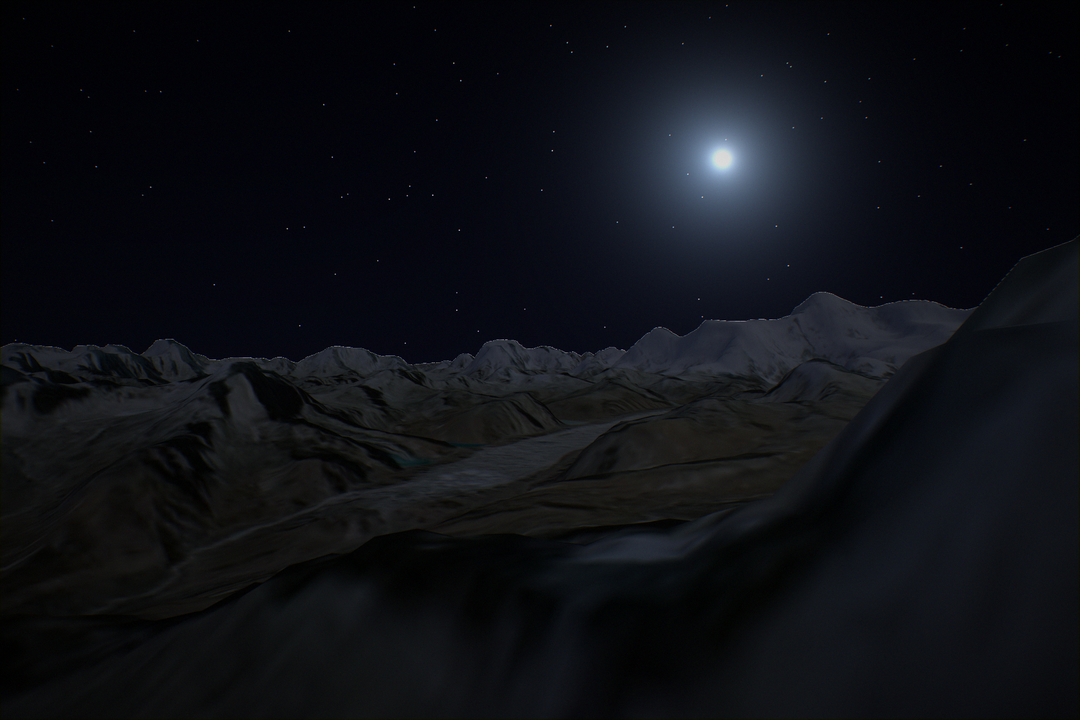
\includegraphics[width=\linewidth]{src/images/input_image.png}
%         \caption{Input photograph}
%     \end{subfigure}
%     \hfill
%     \begin{subfigure}{0.31\textwidth}
%         \centering
%         
\includegraphics[width=\linewidth]{src/images/binary_mask.png}
%         \caption{Predicted mask}
%     \end{subfigure}
%     \hfill
%     \begin{subfigure}{0.31\textwidth}
%         \centering
%         
\includegraphics[width=\linewidth]{src/images/skyline.png}
%         \caption{Extracted skyline}
%     \end{subfigure}

%     \caption{Skyline extraction performed by the proposed system.}
%     \label{fig:skyline_extraction_pipeline}
% \end{figure}

% \section{Skyline Matching Module}

% After skyline extraction, the boundary is converted into an angular profile and compared with the reference database to estimate the camera location. The matching process consists of profile projection, candidate retrieval, fine matching, and location estimation.

% The extracted skyline is first converted from image coordinates into elevation angles using the estimated horizontal field of view and camera geometry. The resulting profile is resampled to the same angular resolution as the reference database so that both profiles can be compared directly.

% The projected skyline is compared with all three reference databases representing visibility distances of \SI{3}{\kilo\meter}, \SI{15}{\kilo\meter}, and \SI{80}{\kilo\meter}. \Gls{fft} (\Gls{fft}) based normalized cross-correlation is used to rapidly evaluate the similarity between the query profile and every reference skyline.

% To reduce the search space, an altitude constraint is applied immediately after the \Gls{fft} stage. Viewpoints whose terrain elevation differs significantly from the estimated camera altitude are excluded before candidate selection. This prevents physically unrealistic matches from entering the refinement stage.

% For each candidate, three skyline descriptors are computed: the skyline profile, its first derivative, and its second derivative. The first derivative describes the local slope of the skyline, while the second derivative highlights changes in skyline curvature.

% \Gls{dtw} (\Gls{dtw}) is then used to compare the combined descriptors while allowing small local variations in skyline shape.
% The candidate with the lowest \Gls{dtw} cost is selected as the final match. The corresponding viewpoint identifier, geographic coordinates, viewing direction, matching confidence, and visibility tier are then returned to the user.

% \begin{table}[H]
% \centering
% \caption{Skyline matching configuration.}
% \label{tab:matching_configuration}

% \begin{tabular}{ll}
% \toprule
% Parameter & Value\\
% \midrule
% Reference viewpoints & 4,920\\
% Visibility tiers & 3\\
% \Gls{fft} shortlist & Top 100 candidates\\
% Angular resolution & $0.25^\circ$\\
% Profile descriptor & Elevation + slope\\
% Final matching & \Gls{dtw}\\
% \bottomrule
% \end{tabular}

% \end{table}



% % \section{Prototype Application}

% % A desktop prototype was developed to integrate all components of the proposed visual geolocation system into a single application. The prototype provides an interface for loading a photograph, extracting the skyline, performing database matching, and displaying the estimated camera location.

% % The application accepts a landscape photograph in JPEG or PNG format. After an image is selected, the skyline extraction module generates a binary mask and extracts the mountain skyline automatically. The extracted profile is then projected into angular coordinates and passed to the skyline matching module.

% % Once the matching process is complete, the application displays the estimated viewpoint together with its geographic coordinates, viewing direction, and matching score. The visibility tier selected during matching is also reported. Figure~\ref{fig:application_interface} shows the main stages of the prototype.

% % The implementation is modular, allowing each stage of the localization pipeline to be tested independently during development. Skyline extraction, database matching, and result visualization are implemented as separate components, making it easier to evaluate individual modules and replace them if improvements are made in the future.
% %
% % \begin{figure}[H]
% % \centering

% % \begin{subfigure}{0.48\textwidth}
% % \centering
% % \includegraphics[width=\linewidth]{src/images/gui_input.png}
% % \caption{Input image}
% % \end{subfigure}
% % \hfill
% % \begin{subfigure}{0.48\textwidth}
% % \centering
% % \includegraphics[width=\linewidth]{src/images/gui_result.png}
% % \caption{Localization result}
% % \end{subfigure}

% % \caption{Prototype application used to perform skyline-based visual geolocation.}
% % \label{fig:application_interface}
% % \end{figure}

% \section{Summary}

% This chapter described the implementation of the proposed visual geolocation system. A reference skyline database was generated from a \Gls{dem} of the Khumbu region, and a synthetic dataset was created to train a lightweight skyline segmentation model. The extracted skyline was matched against the reference database using a hierarchical matching strategy based on \Gls{fft} correlation and \Gls{dtw}. Finally, all components were integrated into a prototype application capable of estimating the location of a mountain photograph.

% \begin{table}[H]
% \centering
% \caption{Main software components used in the implementation.}
% \label{tab:software_components}

% \begin{tabular}{ll}
% \toprule
% Component & Software / Library \\
% \midrule
% Programming language & Python 3 \\
% Terrain ray tracing & HORAYZON (Intel Embree) \\
% Terrain rendering & PyRender \\
% Deep learning & PyTorch \\
% Segmentation model & U-Net (MobileNetV3 encoder) \\
% Image processing & OpenCV, Pillow \\
% Numerical computation & NumPy, SciPy \\
% Coordinate transformation & PyProj \\
% Prototype interface & Tkinter \\
% \bottomrule
% \end{tabular}
% \end{table}
